\chapter{Verification and Results}
\label{chap:results}
The previous chapters described how the LLVM-based $\rho$-VEX compiler has been implemented. In this chapter, we are going to verify the correct operation of the compiler and we are going to measure the performance of the binaries that are generated with the LLVM-based compiler.

\section{Simulation environment}

Benchmarking and verification can be performed using the architecture simulator XSTsim and using the hardware simulator. We have chosen to use the Modelsim hardware simulator because a complete logical simulation of the processor is used for evaluation. Modelsim builds a simulation environment using the $\rho$-VEX VHDL files. A testbench is used to generate test signals. For this simulation the testbench is used to load the instruction and data memory of the $\rho$-VEX processor and to generate correct clock and enable signals to start execution. In Figure \ref{fig:rvex_tb} the testbench process is depicted.

\begin{figure}[ht]
\centering
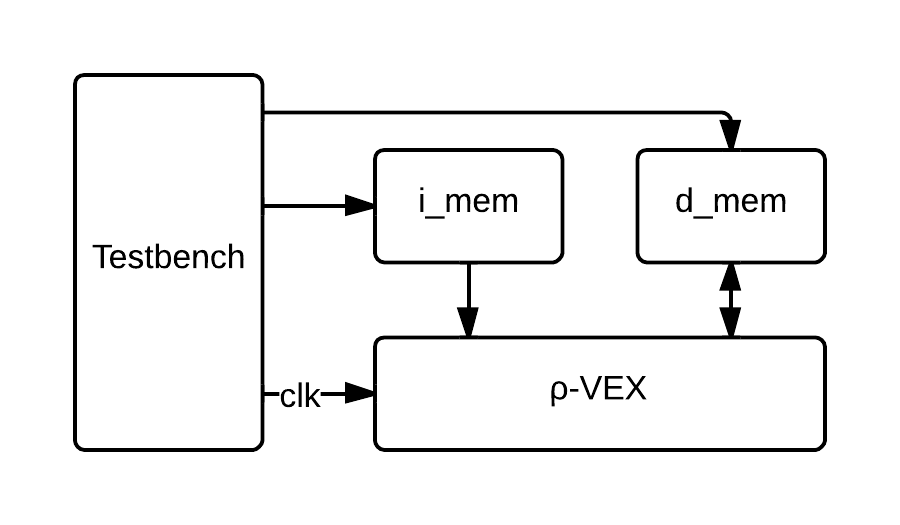
\includegraphics[width=0.8\textwidth]{5_results/img/testbench.png}
\caption{$\rho$-VEX testbench}
\label{fig:rvex_tb}
\end{figure}

Modelsim wave viewer can be used to monitor execution of the processor. The wave viewer has been used to check the contents of the registers and to monitor the instruction pipeline when necessary.

% The architectural simulator has not been used because it only operates on a description of the $\rho$-VEX processor. Bugs that are present in the architectural simulator are not necessarily present in the actual processor. By using the Modelsim simulator we can be sure to a reasonable extent that binaries that execute in Modelsim will also execute on actual hardware. 

\section{Verification}
Unit testing has been used to verify the correct operation of the LLVM compiler. The tests have been performed using the XSTsim simulator and Modelsim. XSTsim can only print pipeline and register information to the terminal. It is not possible to parse strings or information from the program that is executing back to the user. To check if tests are executed correctly we check the return statement after execution of a benchmark. The value in the return register indicates whether the test executed correctly or where at which point the test failed. Using Modelsim the contents of the return register can be monitored during execution.

\begin{itemize}
	\item \textbf{arit.c:} Integer arithmetic tests for \texttt{char}, \texttt{short}, \texttt{int} and \texttt{long long}.
	\item \textbf{if.c:} Integer and boolean comparison operators.
	\item \textbf{float.c:} Testing of floating point library.
	\item \textbf{func.c:} Tests involving pointers and structures.
	\item \textbf{global.c:}  Tests involving global integers, arrays and structures.
	\item \textbf{call.c:} Function calls.
	\item \textbf{func\_pointer.c:} Function calls using function pointers.
	\item \textbf{loop.c:} Basic while loops.
	\item \textbf{misc.c:} Others tests.
\end{itemize}

During preliminary testing of the benchmark additional errors have been found. The verification tests have been updated to catch these errors. Unfortunately, some benchmarking errors are not possible to define as a unit test. Some errors, such as scheduling and register allocation errors, only occur in complex programs. Translating these errors to simple unit tests is not possible because they depend on the higher-level structure of the program.

In addition, the Powerstone benchmark \cite{Jeff-Scott:1998fj} has been used as an additional verification step. The benchmarks consist of a number of programs that test certain functionality. In addition to performance evaluation the benchmarks are also useful to check the executable correctness of the generated binaries.

The following benchmarks have been used for evaluation:

\begin{itemize}
	\item \textbf{adpcm:} codec for voice compression.
	\item \textbf{bcnt:} Bitwise shift and operations on 1K array.
	\item \textbf{blit:} Graphics application
	\item \textbf{compress:} UNIX compression utility
	\item \textbf{crc:} Cyclic redundancy check.
	\item \textbf{DES:} Encryption algorithm.
	\item \textbf{engine:} Engine control application.
	\item \textbf{fir:} Finite Impulse Response filter algorithm.
	\item \textbf{g3fax:} Group 3 fax decode.
	\item \textbf{jpeg:} Image compression algorithm.
	\item \textbf{matrix:} Matrix multiplication.
	\item \textbf{pocsag:} Communication protocol for paging applications.
	\item \textbf{qurt:} Square root calculation using floating-point operations.
	\item \textbf{ucbqsort:} Quicksort algorithm.
	\item \textbf{v42:} Modeom encoding/decoding.
\end{itemize}

These benchmarks have been run using both Modelsim and XSTsim. A number of problems have been found during verification with the Powerstone benchmark. The following benchmarks are not able to execute properly because the benchmark appears to be broken or because the output is not verified.

\begin{itemize}
	\item \textbf{fir:} Algorithm does not execute correctly. The algorithm also fails on a reference workstation. This indicates that the benchmark itself is faulty.
	\item \textbf{des:} Output of algorithm is not verified. This makes it impossible to check if the benchmark was executed correctly.
\end{itemize}

Other benchmarks produce an incorrect result when verifying using Modelsim. These benchmarks produce the expected result when simulation with XSTsim.

\begin{itemize}
	\item \textbf{jpeg:} The jpeg benchmark returns an incorrect result. Manual analysis of the benchmark does not show any errors in scheduling or instruction selection. The algorithm has been further verified by testing subsets of the jpeg algorithm. All the individual subsets work as expected and produce the expected results. Iterating 600 times over each algorithm produces the benchmark result. The code is demonstrated in Listing \ref{lst:bench_jpeg}.



\begin{lstlisting}[language=c, label=lst:bench_jpeg,]

	for (i = 0; i < 600; i++)
		huff_dc_dec(&Data)

	for (i = 0; i < 600; i++)
		huff_ac_dec(&Data);

	for (i = 0; i < 600; i++)
		dquantz_lum(&Data);

	for (i = 0; i < 600; i++)
		j_rev_dct(&Data);

\end{lstlisting}

When the \texttt{for} loop range is changed to a smaller number such as 500 the benchmark produces the expected result. This indicates a possible simulation error where a part of the data memory is overwritten during execution.
	\item \textbf{v42:} This benchmark produces an incorrect result. Manual analysis is not possible because the algorithm is described in a way that makes debugging very difficult. Manual analysis of the output assembly does not indicate any scheduling errors.
\end{itemize}

Because these benchmark are not running correctly we will not consider them for measuring the performance of the LLVM-based compiler.

% FIXME nog een opmerking verwerken van Stephan

\section{Benchmark results}
The Powerstone benchmark has been used to evaluate the performance of the LLVM-based compiler. We measure the execution time of the generated binaries and also the compile-time for each binary. 

\subsection{General performance}
General performance of all the compilers that target the $\rho$-VEX processor are shown in Tables \ref{tbl:LLVM_perf}, \ref{tbl:HP_perf} and \ref{tbl:GCC_perf}. As expected the HP-VEX compiler performs excellent but unfortunately is not able to produce correct executables for higher issue-widths. The GCC compiler has only been implemented for a 4-issue $\rho$-VEX processor.

The absolute performance of the compilers is displayed in Figure \ref{fig:abs_perf}. Table \ref{tbl:LLVM_perf} shows the absolute performance of the LLVM-based compiler. 

\begin{table}
  \centering
    \begin{tabular}{|l|r|r|r|}
    \hline
    \textbf{Benchmark} & \multicolumn{1}{|r|}{\textbf{W2}} & \multicolumn{1}{|r|}{\textbf{W4}}  & \multicolumn{1}{|r|}{\textbf{W8}} \\ \hline
	\texttt{adpcm} 		&  2.206.300	&  2.115.820 	&  2.118.040 	\\ \hline
	\texttt{bcnt} 		&  39.540		&  38.200 		&  35.640 		\\ \hline
	\texttt{blit} 		&  1.164.280	&  1.204.140 	&  1.204.120 	\\ \hline
	\texttt{compress} 	&  3.828.700	&  4.555.420 	&  4.541.900 	\\ \hline
	\texttt{crc} 		&  1.323.160	&  1.290.540 	&  1.290.560 	\\ \hline
	\texttt{engine} 	&  22.820.980	&  18.119.680 	&  18.119.680 	\\ \hline
	\texttt{g3fax} 		&  55.537.540	&  56.645.740 	&  56.680.260 	\\ \hline
	\texttt{matrix} 	&  717.100		&  615.060 		&  615.040 		\\ \hline
	\texttt{pocsag} 	&  2.453.040	&  1.987.140 	&  1.954.860 	\\ \hline
	\texttt{ucbqsort} 	&  9.568.680	&  9.457.160 	&  9.454.600 	\\ \hline
    \end{tabular}
  \caption{LLVM-based compiler performance in ns}
  \label{tbl:LLVM_perf}
\end{table}

\begin{figure}[ht]
\centering
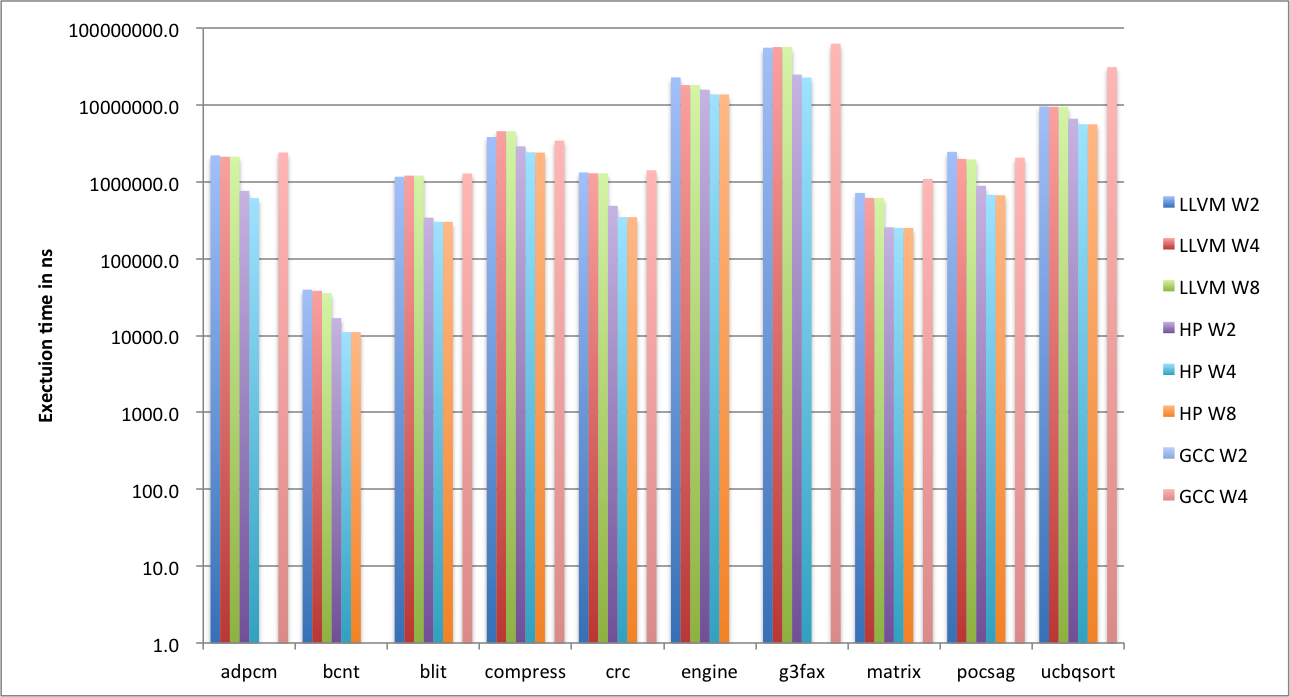
\includegraphics[width=0.8\textwidth]{5_results/img/abs_perf.png}
\caption{Absolute performance}
\label{fig:abs_perf}
\end{figure}

\subsubsection{HP-VEX performance}
In Table \ref{tbl:HP_perf} the absolute performance of the HP-VEX compiler is given. As expected the HP-VEX compiler generates the best performing binaries. Table \ref{tbl:rel_perf} shows that the HP-based compiler binaries are on average twice as fast as the LLVM-based compiler binaries. The LLVM-based compiler offers some speed improvements over the GGC-based compiler for most benchmarks. The HP-VEX compiler is unable to generate working binaries for the \texttt{adpcm} and \texttt{g3fax} benchmark when targeting a 8-issue $\rho$-VEX processor. The reason for this error is not immediately clear.

The HP-VEX compiler generates excellent performing binaries because it has a superiour scheduling techniques for finding and extracting ILP in source code. The HP-VEX compiler uses a trace based scheduling technique which enables better ILP extraction. In addition to this the HP-VEX compiler also seems to do more optimization. Even when compiling with \texttt{-O0} the compiler already performs certain optimizations that are not available for LLVM-based compiler. For example, compare the output for the following simple C program:

\begin{lstlisting}[language=c]
int main() {
	int a = 3, b = 2, c;

	c = a + b;

	return c;
}
	
\end{lstlisting}

Listing \ref{lst:hp_ex} displays the output of the HP-VEX compiler and Listing \ref{lst:llvm_ex} shows the output of the LLVM-based compiler. The output shows immediatly that the HP-VEX compiler has eliminated the add operation and has copied the final value of the operation straight to the return register. The LLVM compiler is only able to perform these kind of operations at higher optimization levels.

\begin{lstlisting}[language=rvex,label=lst:hp_ex, caption={HP compiler output}]

	add $r0.3   = $r0.0, 5  	## Move to return register
;;
	return
;;
\end{lstlisting}

\begin{lstlisting}[language=rvex,label=lst:llvm_ex, caption={LLVM compiler output}]

	add $r0.2 	= $r0.0, 2
	add $r0.3 	= $r0.0, 3	
;;
	add $r0.3   = $r0.2, $r0.3  ## Move to return register
;;
	return
;;
\end{lstlisting}

Figure \ref{fig:rel_HP} shows the relative performance of LLVM-based binaries compared to HP-VEX binaries. Higher then 100\% indicates LLVM-based binaries performing better then HP-VEX binaries. As expected HP-VEX binaries perform better then LLVM-based binaries. Inspection of the generated assembly files indicate that the HP-VEX compiler is able to fill significantly more functional units than the LLVM-based compiler. Further the LLVM-based compiler is overly aggressive in inserting nop instructions to reduce structural and data hazards.

\begin{table}
  \centering
    \begin{tabular}{|l|r|r|r|l|}
    \hline
    \textbf{Benchmark} & \multicolumn{1}{|r|}{\textbf{W2}} & \multicolumn{1}{|r|}{\textbf{W4}}  & \multicolumn{1}{|r|}{\textbf{W8}} & \textbf{Comment} \\ \hline
	\texttt{adpcm} 		&   763.120 	&   613.520 	&   \texttt{ERR} 	& Infinite loop	\\ \hline
	\texttt{bcnt} 		&   16.860 		&   11.100 		&   11.080 			& 	\\ \hline
	\texttt{blit} 		&   341.620 	&   301.360 	&   301.360 		& 	\\ \hline
	\texttt{compress} 	&   2.893.080 	&   2.421.420 	&   2.400.140 		& 	\\ \hline
	\texttt{crc} 		&   486.980 	&   347.040 	&   347.040 		& 	\\ \hline
	\texttt{engine} 	&   15.785.220 	&   13.720.900 	&   13.719.860 		& 	\\ \hline
	\texttt{g3fax} 		&   24.821.120 	&   22.678.220 	&   \texttt{ERR} 	& Infinite loop	\\ \hline
	\texttt{matrix} 	&   255.940 	&   251.260 	&   251.220 		& 	\\ \hline
	\texttt{pocsag} 	&   889.160 	&   676.680 	&   667.880 		& 	\\ \hline
	\texttt{ucbqsort} 	&   6.621.460 	&   5.604.720 	&   5.603.460 		& 	\\ \hline
    \end{tabular}
  \caption{HP-based compiler performance in ns}
  \label{tbl:HP_perf}
\end{table}

\begin{figure}[h]
\centering
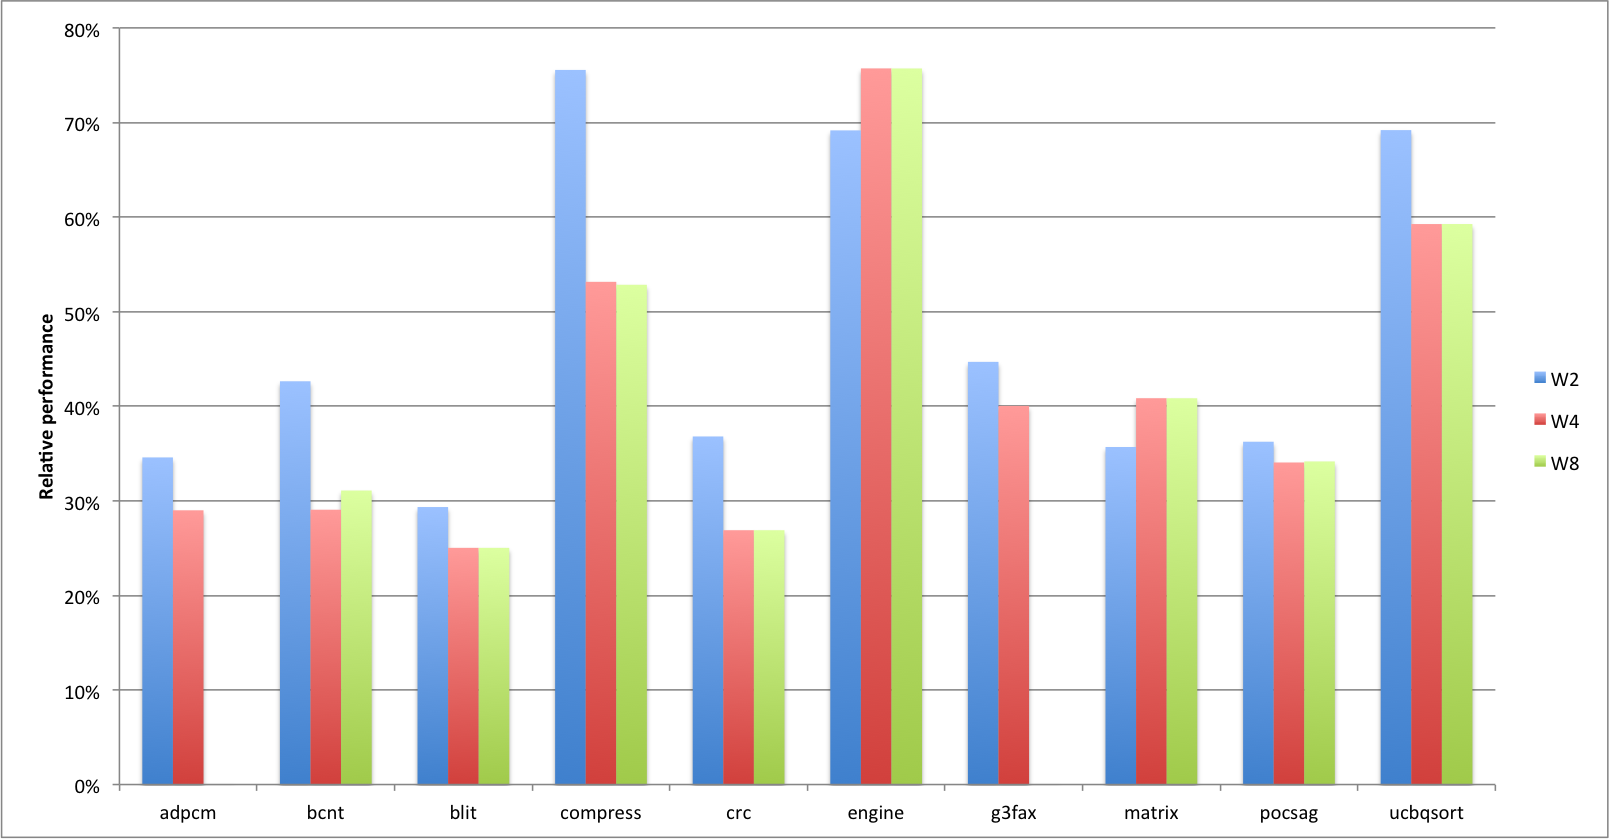
\includegraphics[width=0.8\textwidth]{5_results/img/rel_HP.png}
\caption{HP-LLVM relative performance}
\label{fig:rel_HP}
\end{figure}

\subsubsection{GCC performance}
Table \ref{tbl:GCC_perf} shows the absolute performance of the GCC-based compiler. Figure \ref{fig:rel_GCC} shows the relative performance of LLVM-based binaries compared to GCC-based binaries. The GCC based compiler is unable to compile a number of Powerstone benchmarks. 

Performance of the LLVM-based compiler shows mixed results. Some benchmarks perform significantly better such as \texttt{matrix} and \texttt{ucbqsort} but both compress and pocsag perform worse. Manual inspection of these benchmark do not show a big reason for decreased performance except for the overly aggressive \texttt{nop} insertion of the LLVM machine scheduler.

\begin{table}
  \centering
    \begin{tabular}{|l|r|l|}
    \hline
    \textbf{Benchmark} & \multicolumn{1}{|r|}{\textbf{W4}} & \textbf{Comment} \\ \hline
	\texttt{adpcm} 		& 2.404.760 	&	Wrong result 	\\ \hline
	\texttt{bcnt} 		& \texttt{ERR}	&	Infinite loop	\\ \hline
	\texttt{blit} 		& 1.284.340 	&	Wrong result 	\\ \hline
	\texttt{compress} 	& 3.433.960 	&	\\ \hline
	\texttt{crc} 		& 1.409.960 	&	\\ \hline
	\texttt{engine} 	& \texttt{ERR}	&	Error load		\\ \hline
	\texttt{g3fax} 		& 62.666.300 	&	\\ \hline
	\texttt{matrix} 	& 1.090.420 	&	\\ \hline
	\texttt{pocsag} 	& 2.058.700 	&	\\ \hline
	\texttt{ucbqsort} 	& 31.075.420 	&	\\ \hline
    \end{tabular}
  \caption{GCC-based compiler performance in ns}
  \label{tbl:GCC_perf}
\end{table}


\begin{figure}[ht]
\centering
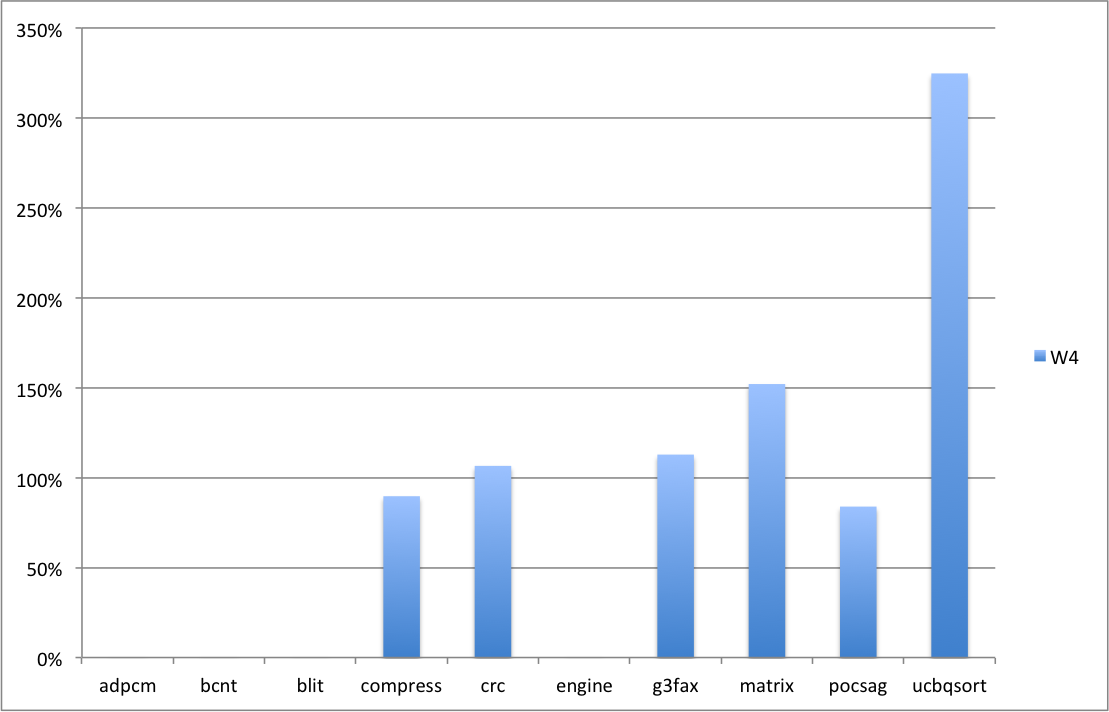
\includegraphics[width=0.8\textwidth]{5_results/img/rel_GCC.png}
\caption{GCC-LLVM relative performance}
\label{fig:rel_GCC}
\end{figure}

\subsubsection{Issue-width}
Close inspection of the absolute performance reveals some interesting facts related to the issue-width of the processor. Increasing the issue-width from 2-issue to 4-issue leads to a significant increase in performance. Further increasing the issue-width to 8-issue machine does not lead to an increase in performance. This is shown in Figure \ref{fig:rel_issue}. For some benchmarks such as \texttt{bcnt} the LLVM-based compiler is able to find extra parallelism but for most benchmarks the performance increase is non-existent.

Manual inspection of the assembly files that are generated shows that both compilers are able to generate instruction packets that use a higher number of functional units. These large instruction packets do not lead to an increase in performance because they are not contained inside loop structures. The amount of times large instruction packets are executed is limited. 

\begin{figure}[ht]
\centering
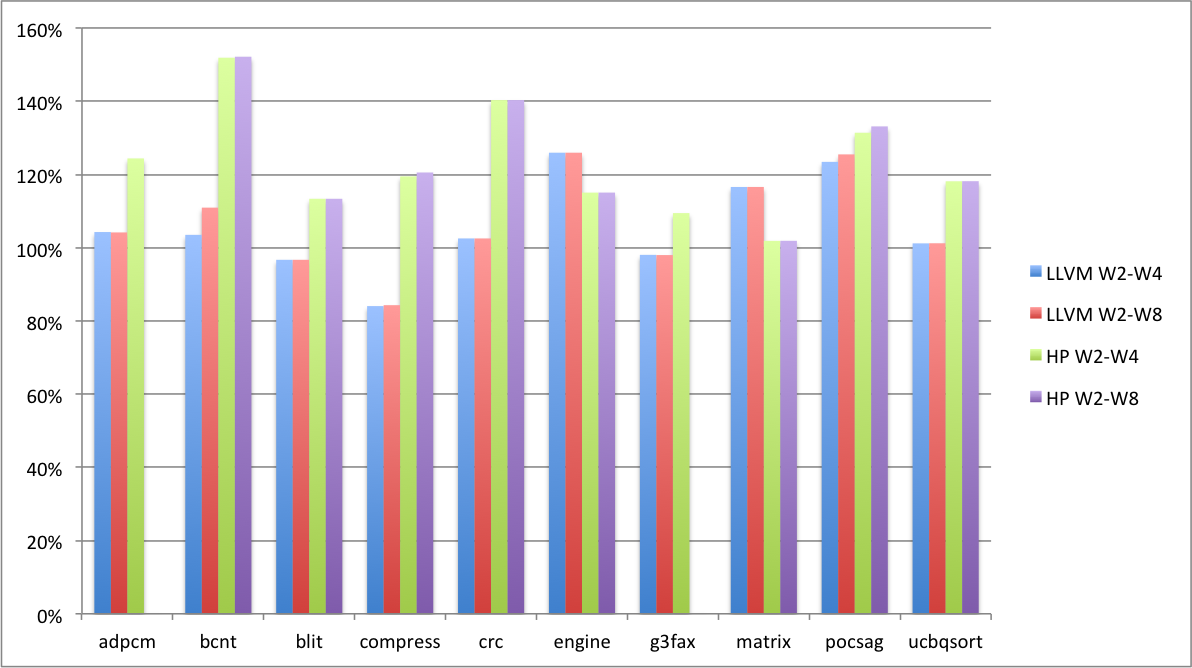
\includegraphics[width=0.8\textwidth]{5_results/img/rel_issue.png}
\caption{Relative performance for increasing issue-width}
\label{fig:rel_issue}
\end{figure}

\begin{table}
  \centering
    \begin{tabular}{|l|r|r|r|l|}
    \hline
    \textbf{Benchmark} & \multicolumn{1}{|r|}{\textbf{VEX W2}} & \multicolumn{1}{|r|}{\textbf{VEX W4}}  & \multicolumn{1}{|r|}{\textbf{VEX W8}} & \textbf{GCC W4} \\ \hline
	\texttt{adpcm} 		&  -65\% &  -71\% & \texttt{ERR} & \texttt{ERR}	\\ \hline
	\texttt{bcnt} 		&  -57\% &  -71\% & -69\% & \texttt{ERR}	\\ \hline
	\texttt{blit} 		&  -71\% &  -75\% & -75\% & \texttt{ERR}	\\ \hline
	\texttt{compress} 	&  -24\% &  -47\% & -47\% & -10\%	\\ \hline
	\texttt{crc} 		&  -63\% &  -73\% & -73\% & 7\%	\\ \hline
	\texttt{engine} 	&  -31\% &  -24\% & -24\% & \texttt{ERR}	\\ \hline
	\texttt{g3fax} 		&  -55\% &  -60\% & \texttt{ERR} & 13\%	\\ \hline
	\texttt{matrix} 	&  -64\% &  -59\% & -59\% & 52\%	\\ \hline
	\texttt{pocsag} 	&  -64\% &  -66\% & -66\% & -16\%	\\ \hline
	\texttt{ucbqsort} 	&  -31\% &  -41\% & -41\% & 225\%	\\ \hline
    \end{tabular}
  \caption{Relative performance of LLVM-compiler binaries}
  \label{tbl:rel_perf}
\end{table}

\subsubsection{Compiler optimizations}
Unfortunately it was not possible to compare the compilers for different optimization levels. The LLVM-based compiler needs a \emph{runtime} library for most benchmarks when compiling with optimizations turned on. This requires us to port the complete LLVM-based \emph{runtime} library to the $\rho$-VEX processor. For this thesis only the floating-point library has been ported. Porting the complete \emph{runtime} library falls outside the scope of this thesis.

\subsection{Generic binary}
The performance of generic binaries has been tested by generating three sets of binaries for a 4-issue $\rho$-VEX processor: Regular binary, Generic binary without optimizations and Generic binary with optimizations. These simulation have been performed with the XSTsim architectural simulator. The relative performance of generic binaries compared to regular binaries is displayed in Figure \ref{fig:rel_gen}.

\begin{figure}[ht]
\centering
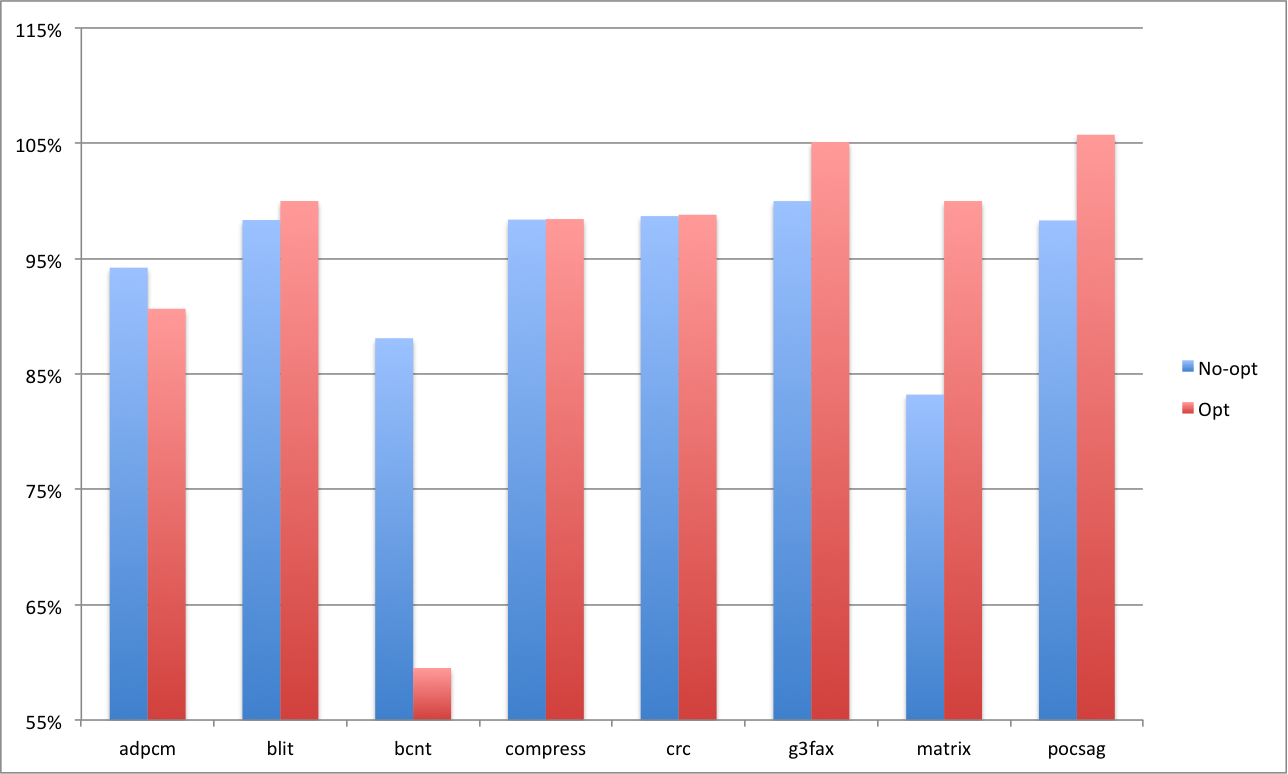
\includegraphics[width=0.8\textwidth]{5_results/img/rel_gen.png}
\caption{Generic-Regular performance}
\label{fig:rel_gen}
\end{figure}

Figure \ref{fig:rel_gen} shows that the optimization for generic binaries provides for more efficient generic binaries for most benchmarks. The \texttt{matrix} benchmark in particular shows excellent increase in performance. The \texttt{adpcm} and \texttt{bcnt} benchmark however shows a significant decrease in performance. Closer inspection of the generated binaries shows that some benchmarks start spending a lot of time executing spill code to save registers to the stack. This is related to the optimization being too aggressive for \texttt{MachineBasicBlocks} with a lot of virtual registers. The optimization causes virtual registers to remain live from the moment they are defined to the end of the \texttt{MachineBasicBlock}. The optimization should be optimized to only keep the virtual register live for the duration of the next instruction packet. This would reduce virtual register usage and would also reduce spill code that is introduced.

Some benchmarks show an increase in performance when compiling using the generic binary optimization. This shows how aggressive the register allocator can be in trying to reduce register pressure. Even though the $\rho$-VEX processor has 64 general purpose registers available the compiler will always try to keep the register usage down to a minimum.  

\begin{table}
  \centering
    \begin{tabular}{|l|r|r|r|r|r|}
    \hline
    \textbf{Benchmark} & \multicolumn{1}{|r|}{\textbf{Regular}} & \multicolumn{1}{|r|}{\textbf{No opt}}  & \multicolumn{1}{|r|}{\textbf{Difference}} & \multicolumn{1}{|r|}{\textbf{With opt}}  & \multicolumn{1}{|r|}{\textbf{Difference}} \\ \hline
	\texttt{adpcm} 		&  176.327 	&	 187.135 	& -6\%	&	 194.492 	& -9\%	\\ \hline
	\texttt{blit} 		&  100.328 	&	 102.007 	& -2\%	&	 100.325 	& 0\%	\\ \hline
	\texttt{bcnt} 		&  3.358  	&	 3.811 		& -12\%	&	 5.643	 	& -40\%	\\ \hline
	\texttt{compress} 	&  385.797 	&	 392.115 	& -2\%	&	 391.920 	& -2\%	\\ \hline
	\texttt{crc} 		&  107.528 	&	 108.950 	& -1\%	&	 108.820 	& -1\%	\\ \hline
	\texttt{g3fax} 		& 5.124.268	& 	 5.124.433	& 0\%	& 	 4.874.923 	& 5\%	\\ \hline
	\texttt{matrix} 	&  51.238 	&	 61.572 	& -17\%	&	 51.238 	& 0\%	\\ \hline
	\texttt{pocsag} 	& 174.128	& 	177.103		& -2\%	& 	 164.661  	& 6\%	\\ \hline
    \end{tabular}
  \caption{Generic binary performance}
  \label{tbl:generic_perf}
\end{table}

\cite{Anthony-Brandon:2013jk} stated that performance should increase if more registers are used for generic binaries. The amount of different registers that are used by each benchmark have been tracked and are displayed in \ref{tbl:gen_regs}. The table shows that the optimization is able to increase the register usage for each benchmark. The \texttt{adpcm} benchmark already uses a large amount of registers and it is not possible to increase this by much. This probably causes the excessive spill code that is generated for this benchmark.

More problematic is the fact that the optimization breaks certain benchmarks. Table \ref{generic_perf} only shows the benchmarks that were able to execute properly. The large number of virtual registers that are used in certain benchmarks are causing unforeseen problems during the compilation process. For instance, during compilation of the \texttt{compress} benchmark the register allocator tried to use the \texttt{PC} register  as a physical register. This was quickly fixed but indicates the kind of problems that are introduced.

\begin{table}
  \centering
    \begin{tabular}{|l|r|r|r|}
    \hline
    \textbf{Benchmark} & \multicolumn{1}{|r|}{\textbf{Regular}} & \multicolumn{1}{|r|}{\textbf{No-opt}} & \multicolumn{1}{|r|}{\textbf{Opt}} \\ \hline
	\texttt{adpcm} 		&   49  &	49 & 	56 \\ \hline
	\texttt{blit} 		&   18  &	18 & 	33 \\ \hline
	\texttt{bcnt} 		&   14  &	14 & 	59 \\ \hline
	\texttt{compress} 	&   27  &	27 & 	60 \\ \hline
	\texttt{crc} 		&   19  &	19 & 	27 \\ \hline
	\texttt{g3fax} 		&   18  &	18 & 	19 \\ \hline
	\texttt{matrix} 	&   18 	&	18 & 	36 \\ \hline
	\texttt{pocsag}		&   24  &	24 & 	31 \\ \hline
    \end{tabular}
  \caption{Register usage}
  \label{tbl:gen_regs}
\end{table}

\subsection{Compile-time}
The compile time has been measured on a virtual machine running \emph{Ubuntu 12.04}. The virtual machine has one processor and 1024MB RAM allocated. The host system uses a 1.7GHz Intel Core i5 processor. The compile-time has been measured by compiling each benchmark 100 times. The Linux \texttt{time} command has been used to measure the execution time.

The HP-VEX and GCC compiler are able to generate assembly files from the input C source code. The LLVM compiler uses a two-phase compilation where Clang is used to compile to LLVM IR and the LLVM static compiler (\texttt{LLC}) is used to compile to assembler. This two-phase compilation will have a negative effect on the performance because extra files need to be read and written from the main memory. This could be avoided by passing the output of Clang straight to \texttt{LLC} but this was not possible to achieve in a timely manner.

The compile-time of each benchmark is given in Table \ref{tbl:compile-time} and depicted in Figure \ref{fig:compile-time}. The GCC-based compiler outperforms both the HP-VEX and LLVM-based compiler in nearly each benchmark. The HP-VEX compiler offers no timing report, which makes it impossible to determine which part of compilation is causing the delay. The lower performance could be related to the extra optimization that the HP-VEX compiler performs. 

The LLVM-based compiler is slower in nearly every benchmark. This could be related to the extra time that is required to write the LLVM IR files to the disk. %FIXME meer uitleg svp

\begin{table}
  \centering
    \begin{tabular}{|l|r|r|r|}
    \hline
    \textbf{Benchmark} & \multicolumn{1}{|r|}{\textbf{HP VEX}} & \multicolumn{1}{|r|}{\textbf{GCC}}  & \multicolumn{1}{|r|}{\textbf{LLVM}} \\ \hline
	\texttt{adpcm} 		& 6,41 & 6,55 & 5,68 \\ \hline
	\texttt{bcnt} 		& 1,72 & 2,02 & 2,91 \\ \hline
	\texttt{blit} 		& 2,26 & 2,12 & 3,72 \\ \hline
	\texttt{compress} 	& 8,82 & 7,19 & \\ \hline
	\texttt{crc} 		& 2,54 & 2,30 & 3,28 \\ \hline
	\texttt{engine} 	& 5,60 & 3,64 & 4,14 \\ \hline
	\texttt{g3fax} 		& 5,00 & 3,95 & 6,58 \\ \hline
	\texttt{matrix} 	& 1,97 & 1,88 & 2,92 \\ \hline
	\texttt{pocsag} 	& 6,60 & 4,28 & 5,49 \\ \hline
	\texttt{qurt}	 	& 2,74 & 3,46 & 3,33 \\ \hline
	\texttt{ucbqsort} 	& 8,41 & 3,60 & 4,54 \\ \hline
    \end{tabular}
  \caption{Compile-time in seconds}
  \label{tbl:compile-time}
\end{table}

\begin{figure}[ht]
\centering
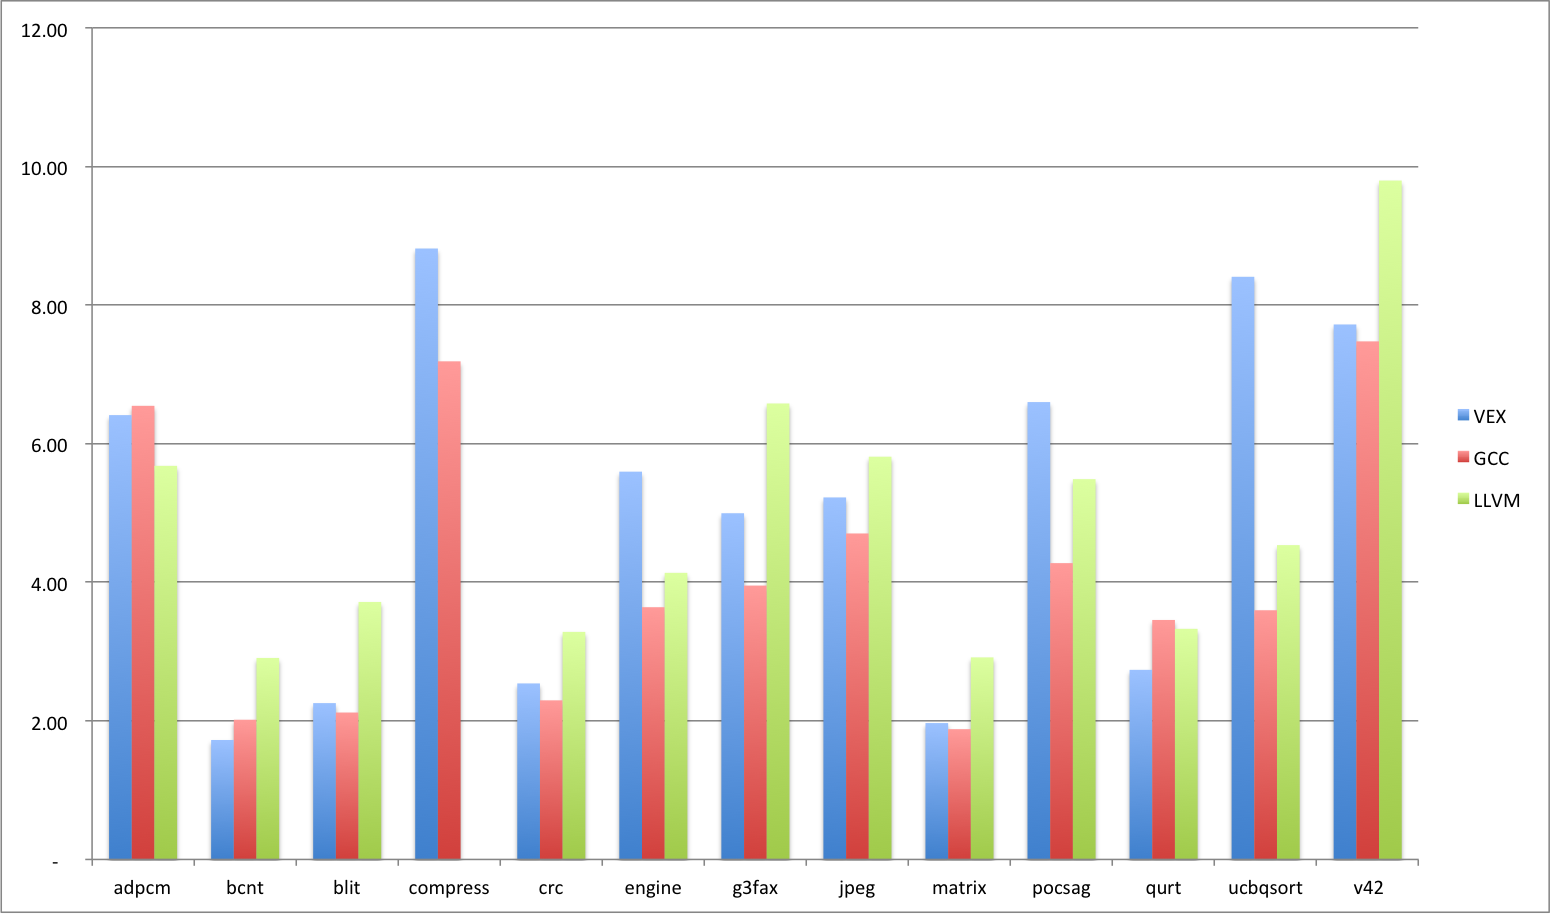
\includegraphics[width=0.8\textwidth]{5_results/img/compile-time.png}
\caption{Compile-time in seconds}
\label{fig:compile-time}
\end{figure}

\section{Conclusion}
In this section we have shown how the operation of the LLVM-based compiler has been verified and how well binaries execute that have been generated with the LLVM-based compiler.

The benchmarks and verifications have shown that the LLVM-based compiler still contains bugs. Not all benchmarks are able to execute using the Modelsim simulator but all benchmarks are able to execute using the XSTsim simulator. This indicates that there are probably scheduling issues in the assembly that is generated. The reason for the failing benchmarks remain unclear. It is possible that the compiler generates code that is not scheduled properly but analysis of the \texttt{jpeg} benchmark indicated the possibility of other issues. 

We have shown that the LLVM-based compiler exceeds the performance of the GCC-based compiler but the compiler is still outperformed by the HP-VEX compiler. As expected the HP-VEX compiler generates binaries that perform very well. This is related to the trace based scheduling techniques that are employed to extract a high level of ILP \cite{Lowney:1993qy}. In addition, the HP-VEX compiler also performs certain optimizations that are not available to the LLVM-based compiler at \texttt{-O0}.

Additionally, the benchmarks have also shown that the LLVM-based compiler is the only compiler able to generate correct code for all selected benchmarks. Surprisingly, even the HP-VEX compiler generates incorrect binaries for certain benchmarks. The code quality of the GCC-based compiler is bad with four benchmarks failing to execute.

Furthermore, we have also shown that the generic binary optimization allows generic binaries to operate at speeds that are nearly equal to the regular binaries. The generic binary optimization does introduce spill code in benchmarks that already use a large number of physical registers. The current optimization is too aggressive for the \texttt{adpcm} benchmark and introduces excessive amount of spill code that degrades performance. The optimization should be fine tuned to consider this situation. More problematic is the fact that the used optimization breaks certain benchmarks.

\acresetall
